
%%%%%%%%%%%%%%%%%%%%%%%%%%%%%%%%%%%%%%%%%%%%%%%%%%%%%%%%%%%%%%%%%%%%%%%%%%%%
%% main.tex
%%
%% Content file for an Internal Research Report.
%% Doctoral Program in Engineering Sciences at ITESO.
%%
%% Class: iteso-irr (see iteso-irr.cls and iteso-phdengsci.def)
%% Compile with: pdflatex -> bibtex -> pdflatex -> pdflatex
%%
%% This work may be distributed and/or modified under the
%% conditions of the LaTeX Project Public License
%%%%%%%%%%%%%%%%%%%%%%%%%%%%%%%%%%%%%%%%%%%%%%%%%%%%%%%%%%%%%%%%%%%%%%%%%%%%

\documentclass{iteso-irr}

%% --- Report metadata (edit for each new report) -------------------------

\ReportTitle{%
  An Updated and Open Sourced \LaTeX{} Template for Internal Research
  Reports of the Doctoral Program in Engineering Sciences at ITESO}
\ReportAuthors{J. Francisco Munoz-Elguez\'{a}bal}
\ReportFileName{PhDEngScITESO-26-00-R}
\ReportDate{Mar 31, 2026}
\CopyrightYear{2026}

%% Filename convention: PhDEngScITESO-YY-NN-R
%%   YY = last two digits of year of publication (approval date)
%%   NN = consecutive number assigned by the Chair of the PhD program

\begin{document}

%%%%%%%%%%%%%%%%%%%%%%%%%%%%%%%%%%%%%%%%%%%%%%%%%%%%%%%%%%%%%%%%%%%%%%%%%%%%
%% COVER PAGE (includes blank verso for twoside printing)
%%%%%%%%%%%%%%%%%%%%%%%%%%%%%%%%%%%%%%%%%%%%%%%%%%%%%%%%%%%%%%%%%%%%%%%%%%%%

\makecoverpage

%%%%%%%%%%%%%%%%%%%%%%%%%%%%%%%%%%%%%%%%%%%%%%%%%%%%%%%%%%%%%%%%%%%%%%%%%%%%
%% FIRST PAGE: Title, Authors, Keywords, Abstract
%%%%%%%%%%%%%%%%%%%%%%%%%%%%%%%%%%%%%%%%%%%%%%%%%%%%%%%%%%%%%%%%%%%%%%%%%%%%

\setcounter{page}{1}

\makefirstpage
{% --- Keywords ---
  copyright, format, internal report, \LaTeX{}, Overleaf, BibTeX,
  figures, references, research report, template%
}
{% --- Abstract ---
  An updated and open sourced \LaTeX{} template to write formal internal
  research reports for the PhD Program in Engineering Sciences at ITESO
  is presented. It provides a custom document class (\texttt{iteso-irr})
  compatible with Overleaf, implementing the institutional formatting
  standard: automated cover page and title page generation, Roman-numeral
  section numbering, IEEE-style captions and citation format, and
  BibTeX-based bibliography management with Zotero integration. The
  template separates content from presentation, allowing authors to focus
  on technical writing while the class enforces consistent formatting
  across all reports in the doctoral program.%
}
{% --- Funding footnote ---
  This work was supported in part by SECIHTI (Secretar\'{i}a de Ciencia,
  Humanidades, Tecnolog\'{i}a e Innovaci\'{o}n) through the recognition
  granted to the PhD Program in Engineering Sciences at ITESO.%
}

%%%%%%%%%%%%%%%%%%%%%%%%%%%%%%%%%%%%%%%%%%%%%%%%%%%%%%%%%%%%%%%%%%%%%%%%%%%%
%% I. INTRODUCTION
%%%%%%%%%%%%%%%%%%%%%%%%%%%%%%%%%%%%%%%%%%%%%%%%%%%%%%%%%%%%%%%%%%%%%%%%%%%%

\section{Introduction}
\label{sec:introduction}

On a first note, this template is based on the formatting standard established by the
internal research reports template originally developed by
Rayas-S\'{a}nchez for the CAECAS research group at ITESO
\cite{ref:rayas2015word}, later adopted as the official format for the
Doctoral Program in Engineering Sciences. The present \LaTeX{}
implementation preserves the same structural and typographic conventions
while leveraging automated cross-referencing, bibliography management,
and consistent compilation through Overleaf.

In order to make consistent progress on a research line, it is extremely
important to make rigorous documentation of every significant step forward.
Documenting internal research reports is particularly important within a
group of people. Most researchers tend to be quite disorganized with their
paper work. Usually, they create many handwriting notes, provisional
word-processing files, scripts, and diagrams for each project they develop.
After some time (a few months or even a few weeks) it is very difficult to
find, understand, and re-use such documented material.

Writing formal internal reports is also important to show evidence on
research progress to other organizations. In Mexico, for instance, SECIHTI
requires formal internal reports to most research groups that are granted
significant research funding. In addition, by having an official internal
report we can more easily deal with intellectual property and copyright
issues.

Internal reports do not have to be long. A report might consist of just 5
or 6 pages, including cover page and figures. What is most important of an
internal research report is its accuracy in terms of contents and
consistency in terms of format. Making research is similar to building a
house: it is realized by assembling many simple building blocks. Each
building block must be robust and well built. Similarly, every internal
report must have been extensively reviewed and revised, so that it becomes a
useful piece of knowledge for further research work.

By having a simple and well-defined template for writing research reports,
authors can focus their attention on the technical issues (logical
argumentation, clarity, precision, consistency, etc.) and writing aspects
(grammar, spelling, punctuation, etc.), since most of the formatting is
realized semi-automatically. A suitable template should facilitate
allocating figures and formatting equations and references.

This report describes the format and style that must be used for internal
research reports in the Doctoral Program in Engineering Sciences at ITESO,
particularly to document progress in the Seminarios IDI (Seminars on
Research, Development, and Innovation) for this PhD program.

The internal research reports for the PhD Program in Engineering Sciences
at ITESO must be written in English, to facilitate sharing information and
scientific publishing. It should also be noticed that text in other
languages different to English must be typed either between quotation marks,
or using italics (e.g., see footnote on previous page).

%%%%%%%%%%%%%%%%%%%%%%%%%%%%%%%%%%%%%%%%%%%%%%%%%%%%%%%%%%%%%%%%%%%%%%%%%%%%
%% II. USING LATEX STYLES
%%%%%%%%%%%%%%%%%%%%%%%%%%%%%%%%%%%%%%%%%%%%%%%%%%%%%%%%%%%%%%%%%%%%%%%%%%%%

\section{Using \LaTeX{} Styles}
\label{sec:styles}

This template uses a custom document class, \texttt{iteso-irr}, which
encapsulates all formatting rules. Each structural element of the document
is handled by a specific \LaTeX{} command or environment. Normal text is
typeset using the default body font and paragraph settings, while the
Roman-numbered section titles are produced by the \verb|\section{}|
command. Subsections use the \verb|\subsection{}| command and are labeled
with capital letters.

When a portion of text is copied from another file, it can be pasted
directly. \LaTeX{} will automatically apply the formatting defined in
this template. In other words, authors write plain text with standard
\LaTeX{} markup in \texttt{main.tex}, and the class file enforces the
institutional format. No manual formatting of fonts, margins, headers,
or caption styles is needed.

%%%%%%%%%%%%%%%%%%%%%%%%%%%%%%%%%%%%%%%%%%%%%%%%%%%%%%%%%%%%%%%%%%%%%%%%%%%%
%% III. DOCUMENT STRUCTURE
%%%%%%%%%%%%%%%%%%%%%%%%%%%%%%%%%%%%%%%%%%%%%%%%%%%%%%%%%%%%%%%%%%%%%%%%%%%%

\section{Document Structure}
\label{sec:structure}

The present template provides all the necessary commands for structuring
the document. The cover page is produced by \verb|\makecoverpage|, and the
first page (with keywords, abstract, and funding acknowledgment) is
produced by \verb|\makefirstpage|.

Report metadata is declared once in the preamble of \texttt{main.tex}
through commands such as \verb|\ReportTitle|, \verb|\ReportAuthors|,
\verb|\ReportFileName|, \verb|\ReportDate|, and \verb|\CopyrightYear|.
All occurrences throughout the document (cover page, title page, headers,
footers) are updated automatically upon recompilation.

%%%%%%%%%%%%%%%%%%%%%%%%%%%%%%%%%%%%%%%%%%%%%%%%%%%%%%%%%%%%%%%%%%%%%%%%%%%%
%% IV. INITIAL PAGES
%%%%%%%%%%%%%%%%%%%%%%%%%%%%%%%%%%%%%%%%%%%%%%%%%%%%%%%%%%%%%%%%%%%%%%%%%%%%

\section{Initial Pages}
\label{sec:initial}

\subsection{The Cover Page}
\label{sec:coverpage}

The cover page contains the report title, author name(s), the filename
identifier, the date and location, the institutional affiliation, the
ITESO logo, and the copyright notice. The filename follows the convention
\texttt{PhDEngScITESO-YY-NN-R}, where \texttt{YY} corresponds to the
last two digits of the year of publication and \texttt{NN} corresponds
to a consecutive number assigned by the Chair of the PhD program.

To insert the ITESO logo, place the image file (e.g.,
\texttt{iteso-logo.png}) in the \text{style/} project directory and uncomment the
corresponding \verb|\includegraphics| line in the cover page definition
inside \texttt{iteso-phdengsci.def}.

\subsection{The First Page}
\label{sec:firstpage}

The first page automatically displays the title, authors, institutional
contact information, keywords, and abstract. When the reported research
work has been supported financially, the corresponding credit is given
using a footnote attached to the abstract header. The funding text is
passed as the third argument to \verb|\makefirstpage|.

Keywords are one-word or two-word expressions representing the main topics
addressed in the report. All keywords should be in lower-case, except
proper names and acronyms.

%%%%%%%%%%%%%%%%%%%%%%%%%%%%%%%%%%%%%%%%%%%%%%%%%%%%%%%%%%%%%%%%%%%%%%%%%%%%
%% V. INSERTING EQUATIONS AND MATHEMATICAL SYMBOLS
%%%%%%%%%%%%%%%%%%%%%%%%%%%%%%%%%%%%%%%%%%%%%%%%%%%%%%%%%%%%%%%%%%%%%%%%%%%%

\section{Inserting Equations and Mathematical Symbols}
\label{sec:equations}

All mathematical symbols must be italic, including Greek letters. Vectors
and matrices must be bold italic, and scalars must use regular italic font
(not bold). This is an example of a linear system:
%
\begin{equation}
  \bm{A}\bm{y} + b\bm{z} = \bm{c}
  \label{eq:linear_system}
\end{equation}
%
\noindent where $\bm{A} \in \Re^{n \times m}$,
$\bm{y} \in \Re^{m}$,
$\bm{z}$ and $\bm{c} \in \Re^{n}$,
$b \in \Re$.
Notice that the mathematical expressions in this paragraph are inserted
as inline math and not as plain text. This ensures consistent font style
with the displayed equations.

An example from machine learning is the regularized empirical risk
minimization objective:
%
\begin{equation}
  \bm{\theta}^{*}
  = \arg\min_{\bm{\theta}}
    \frac{1}{N} \sum_{i=1}^{N}
    \mathcal{L}\!\left(f(\bm{x}^{(i)}; \bm{\theta}),\, y^{(i)}\right)
    + \lambda \|\bm{\theta}\|_2^2
  \label{eq:erm}
\end{equation}
%
\noindent where $\bm{\theta} \in \Re^{d}$ contains the model parameters,
$\{(\bm{x}^{(i)}, y^{(i)})\}_{i=1}^{N}$ is the training set,
$\mathcal{L}$ denotes the loss function,
$f(\cdot\,; \bm{\theta})$ is the model, and
$\lambda \geq 0$ controls the strength of $L_2$ regularization.

Numbered equations use the \texttt{equation} environment, as in
\eqref{eq:linear_system} and \eqref{eq:erm}, so that they are centered
and the equation number is aligned to the right. To refer to an equation,
use \verb|\eqref{}|. For example: ``from \eqref{eq:linear_system} we
obtain\ldots'', instead of ``from equation 1 we obtain\ldots''.

Simple mathematical expressions can be typed directly as part of the text
body using inline math mode, as long as they do not need to be referenced
later. An example: $\beta = \alpha / (1 - \alpha)$.

%%%%%%%%%%%%%%%%%%%%%%%%%%%%%%%%%%%%%%%%%%%%%%%%%%%%%%%%%%%%%%%%%%%%%%%%%%%%
%% VI. FIGURES AND TABLES
%%%%%%%%%%%%%%%%%%%%%%%%%%%%%%%%%%%%%%%%%%%%%%%%%%%%%%%%%%%%%%%%%%%%%%%%%%%%

\clearpage

\section{Figures and Tables}
\label{sec:figures_tables}

\begin{table}[t]
  \centering
  \caption{Summary of Reference Types and Their Formats}
  \label{tab:reference_types}
  \begin{tabular}{l l}
    \toprule
    \textbf{Reference Type} & \textbf{Example Citation} \\
    \midrule
    Journal papers               & \cite{ref:lecun2015} \\
    Books                        & \cite{ref:goodfellow2016} \\
    Book chapters                & \cite{ref:rayas2013ch} \\
    Conference papers (ML)       & \cite{ref:he2016resnet} \\
    Conference papers (Eng.)     & \cite{ref:rayas2004conf} \\
    arXiv preprints              & \cite{ref:vaswani2017attention} \\
    Technical reports            & \cite{ref:openai2023gpt4} \\
    Datasets                     & \cite{ref:deng2009imagenet} \\
    Software repositories        & \cite{ref:pytorch2019} \\
    Open source software         & \cite{ref:python} \\
    Internal research reports    & \cite{ref:rayas2015word} \\
    \bottomrule
  \end{tabular}
\end{table}

\begin{table}[t]
  \centering
  \caption{Example of an Experimental Results Table}
  \label{tab:results_example}
  \begin{tabular}{l c c c}
    \toprule
    \textbf{Method} & \textbf{Accuracy (\%)} & \textbf{F1 Score}
                    & \textbf{Time (s)} \\
    \midrule
    Baseline SVM       & $82.3 \pm 0.5$ & $0.791 \pm 0.008$ & 12.4 \\
    Random Forest      & $85.1 \pm 0.4$ & $0.823 \pm 0.006$ & 8.7 \\
    Neural Network     & $\mathbf{89.7 \pm 0.3}$ & $\mathbf{0.881 \pm 0.004}$
                       & 45.2 \\
    \bottomrule
  \end{tabular}
\end{table}

\subsection{Tables}
\label{sec:tables}

In \LaTeX{}, figures and tables are handled as floating environments
that are automatically placed by the typesetting engine within the
main document. Placement can be influenced through optional specifiers
(\texttt{h}, \texttt{t}, \texttt{b}, \texttt{p}) passed to the
environment.

Tables are always shown at the beginning of the file containing figures 
and tables, and are numbered using Roman numerals. Their captions are 
placed above the table and use small capitals. Table~\ref{tab:reference_types}
illustrates the standard format for citation examples. For the case of having 
two or more tables to shown, it might be needed a \verb|\clearpage| command 
to start the section or subsection in a new page. And, When presenting 
experimental results, it is conventional to bold-face the best result in 
each column and to report uncertainty as mean $\pm$ standard
deviation. Table~\ref{tab:results_example} shows the recommended format. Also, 
The text included within a table must be horizontally and vertically
centered. Regular rows do not use visible horizontal lines beyond the
header and footer rules. Columns should never use visible vertical lines.

\begin{figure}[t]
    \centering
    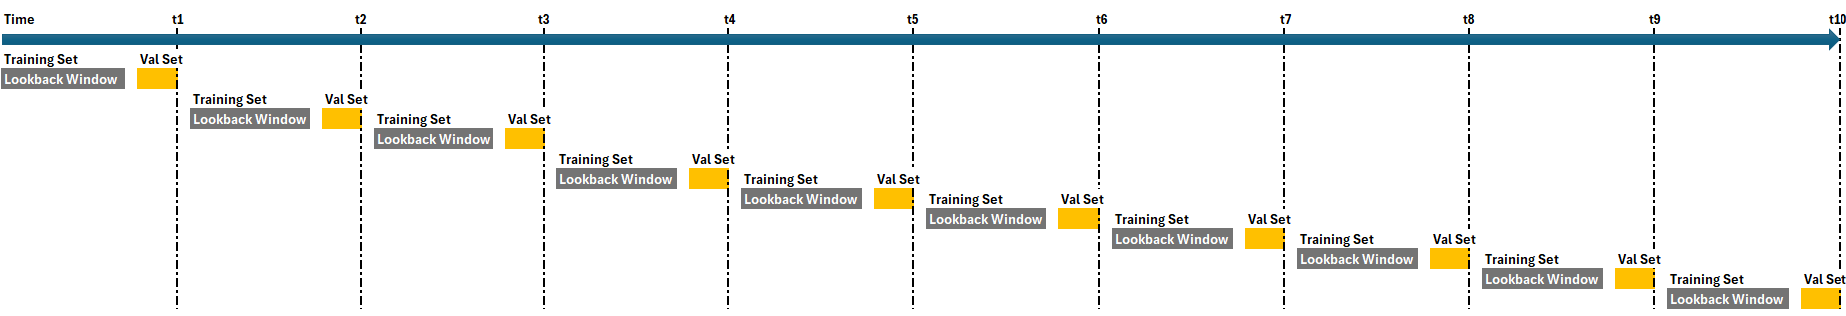
\includegraphics[width=0.80\columnwidth]{figures/figure_1.png}
    \caption{Example figure showing typical format for plots}
    \label{fig:example}
\end{figure}

\subsection{Figures}
\label{sec:figures}

Each figure must have a descriptive caption (as self-contained as
possible), so that the reader can understand the work by examining the
figures and reading their captions. Figures are inserted using the
\texttt{figure} environment and the \verb|\includegraphics| command, as it 
can be appreciated in with the Fig~\ref{fig:example}, which is a wide horizontally 
oriented plot. 

% Example figure (uncomment and provide actual image file):
% \begin{figure}[htbp]
%   \centering
%   \includegraphics[width=0.8\columnwidth]{example-figure.pdf}
%   \caption{Example figure showing the typical format for plots.
%     All text labels in plots should use Times font. The font size for
%     axis numbers is slightly smaller than the font size used for labels.}
%   \label{fig:example}
% \end{figure}

When inserting figures with multiple images, use the \texttt{subcaption}
package with the \texttt{subfigure} environment, providing identifiers
(a), (b), etc., for each sub-image.

\subsection{Inserting Figures from Matlab}
\label{sec:matlab_figures}

Figures created in Matlab should be exported in vector format (PDF or
EPS) for best results in \LaTeX{}. The recommended Matlab commands are:
%
\begin{lstlisting}[language=Python, caption={Exporting a matplotlib
    figure to PDF.}, label={lst:matplotlib_export}]
  print('-dpdf', 'figure_name.pdf')
  % or
  exportgraphics(gcf, 'figure_name.pdf', ...
      'ContentType', 'vector')
\end{lstlisting}
%
All plots should be distinguishable in both color and black-and-white
printing, by using not only different colors but also different line
styles and markers.

\subsection{Inserting Figures from Python and R}
\label{sec:python_figures}

Figures created with Python's \texttt{matplotlib} or \texttt{seaborn}
libraries should be saved in PDF format for vector quality:
%
\begin{lstlisting}[language=Python, caption={Exporting a matplotlib
    figure to PDF.}, label={lst:matplotlib_export}]
import matplotlib.pyplot as plt

fig, ax = plt.subplots()
ax.plot(x, y, label='Training loss')
ax.set_xlabel('Epoch')
ax.set_ylabel('Loss')
ax.legend()
fig.savefig('figure_name.pdf', bbox_inches='tight')
\end{lstlisting}

\clearpage

For R, the equivalent export using \texttt{ggplot2} is:
%
\begin{lstlisting}[language=R, caption={Exporting a ggplot2 figure
    to PDF.}, label={lst:ggplot_export}]
library(ggplot2)
p <- ggplot(data, aes(x = epoch, y = loss)) +
     geom_line() +
     labs(x = "Epoch", y = "Loss")
ggsave("figure_name.pdf", plot = p,
       width = 6, height = 4)
\end{lstlisting}

Figures generated inside Jupyter notebooks can be saved to PDF
programmatically by calling \texttt{fig.savefig()} in the cell that
produces the plot. The saved PDF file is then included in the \LaTeX{}
project via \verb|\includegraphics| as with any other figure.

\subsection{Inserting Figures from Other Tools}
\label{sec:other_figures}

Figures created with drawing tools such as Visio, Inkscape, or
\texttt{draw.io} should be exported in vector format (PDF or SVG)
before inclusion. PDF is the preferred format for \texttt{pdflatex}
compilation. If only SVG is available, convert it to PDF using
Inkscape on the command line:
%
\begin{verbatim}
  inkscape --export-type=pdf figure_name.svg
\end{verbatim}
%
Bitmap formats (PNG, JPEG) should be used only when no vector
alternative exists, such as photographs or screenshots. Bitmap
figures consume more memory and lose resolution when scaled.

\subsection{Creating Figures with TikZ and PGFPlots}
\label{sec:tikz_figures}

For figures that must match the document font exactly (architecture
diagrams, flowcharts, training curves), the \texttt{tikz} and
\texttt{pgfplots} packages allow figures to be defined directly in
\LaTeX{} source code. This approach produces figures whose labels,
symbols, and fonts are rendered by the same typesetting engine as the
body text. The \texttt{tikz} and \texttt{pgfplots} packages are not
loaded by default in this template to avoid increasing compilation time
for reports that do not use them. To enable them, add the following
lines in the preamble of \texttt{main.tex}:
%
\begin{lstlisting}
  \usepackage{tikz}
  \usepackage{pgfplots}
  \pgfplotsset{compat=1.18}
\end{lstlisting}

%%%%%%%%%%%%%%%%%%%%%%%%%%%%%%%%%%%%%%%%%%%%%%%%%%%%%%%%%%%%%%%%%%%%%%%%%%%%
%% VII. ALGORITHMS AND CODE LISTINGS
%%%%%%%%%%%%%%%%%%%%%%%%%%%%%%%%%%%%%%%%%%%%%%%%%%%%%%%%%%%%%%%%%%%%%%%%%%%%

\section{Algorithms and Code Listings}
\label{sec:algorithms}

\subsection{Algorithm Pseudocode}
\label{sec:pseudocode}

The \texttt{algorithm2e} package (loaded by the document class) provides
a structured environment for presenting algorithms. Algorithms are
numbered independently of equations and figures, and can be referenced
with \verb|\label{}| and \verb|\ref{}|.

Algorithm~\ref{alg:sgd} shows an example of stochastic gradient descent
in the format expected for internal research reports.

\begin{algorithm}[htbp]
\SetAlgoLined
\KwIn{Training set $\mathcal{D} = \{(\bm{x}^{(i)}, y^{(i)})\}_{i=1}^{N}$,
      learning rate $\eta$, number of epochs $T$}
\KwOut{Trained parameters $\bm{\theta}$}
Initialize $\bm{\theta}$ randomly\;
\For{$t \leftarrow 1$ \KwTo $T$}{
  Shuffle $\mathcal{D}$\;
  \For{each mini-batch $\mathcal{B} \subset \mathcal{D}$}{
    Compute gradient $\bm{g} \leftarrow
      \frac{1}{|\mathcal{B}|}\sum_{(\bm{x},y) \in \mathcal{B}}
      \nabla_{\bm{\theta}}
      \mathcal{L}(f(\bm{x};\bm{\theta}), y)$\;
    Update $\bm{\theta} \leftarrow \bm{\theta} - \eta\,\bm{g}$\;
  }
}
\Return{$\bm{\theta}$}\;
\caption{Mini-Batch Stochastic Gradient Descent}
\label{alg:sgd}
\end{algorithm}

The key elements demonstrated above are: \verb|\KwIn| and \verb|\KwOut|
for specifying inputs and outputs, \verb|\For| for loop constructs,
mathematical notation within the pseudocode body, and
\verb|\caption| plus \verb|\label| for referencing. Conditional
constructs use \verb|\If|, \verb|\ElseIf|, and \verb|\Else|. The
\texttt{algorithm2e} documentation provides the full set of available
constructs.

\subsection{Source Code Listings}
\label{sec:code_listings}

The \texttt{listings} package (loaded by the document class) provides
formatted source code blocks with syntax highlighting and line numbers.
Listings are appropriate when the exact implementation matters, such as
a data preprocessing pipeline or a model architecture definition.
Listing~\ref{lst:pytorch_model} shows an example.

\begin{lstlisting}[language=Python,
    caption={A simple feedforward neural network in PyTorch.},
    label={lst:pytorch_model}]
import torch
import torch.nn as nn

class SimpleNet(nn.Module):
    def __init__(self, input_dim, hidden_dim, output_dim):
        super().__init__()
        self.fc1 = nn.Linear(input_dim, hidden_dim)
        self.relu = nn.ReLU()
        self.fc2 = nn.Linear(hidden_dim, output_dim)

    def forward(self, x):
        x = self.relu(self.fc1(x))
        return self.fc2(x)
\end{lstlisting}

The \texttt{lstset} defaults (defined in \texttt{iteso-phdengsci.def})
provide a single-frame style with line numbers. These defaults can be
overridden per listing through optional parameters in the
\verb|\begin{lstlisting}| environment.

For short inline code references within the text body, use
\verb|\texttt{}| for identifiers (e.g., \texttt{nn.Module}) or
\verb|\lstinline| for syntax-highlighted fragments (e.g.,
\lstinline[language=Python]{def forward(self, x):}).

%%%%%%%%%%%%%%%%%%%%%%%%%%%%%%%%%%%%%%%%%%%%%%%%%%%%%%%%%%%%%%%%%%%%%%%%%%%%
%% VIII. MAKING REFERENCES
%%%%%%%%%%%%%%%%%%%%%%%%%%%%%%%%%%%%%%%%%%%%%%%%%%%%%%%%%%%%%%%%%%%%%%%%%%%%

\section{Making References}
\label{sec:references}

It is very important to make proper reference to relevant work of other
authors, as well as to our own previous related work. The format used in
the PhD Program in Engineering Sciences at ITESO is the IEEE citation
reference format \cite{ref:ieee_guide}.

The following are examples of the format for different types of references:
%
\begin{letterlist}
  \item Journal papers: \cite{ref:rayas2006}, \cite{ref:lecun2015}.
  \item Books: \cite{ref:goodfellow2016}, \cite{ref:bishop2006}.
  \item Book chapters: \cite{ref:rayas2013ch}, \cite{ref:rayas2013ch2}.
  \item Conference papers (engineering): \cite{ref:rayas2004conf},
        \cite{ref:gutierrez2006conf}.
  \item Conference papers (ML venues): \cite{ref:he2016resnet},
        \cite{ref:devlin2019bert}.
  \item arXiv preprints: \cite{ref:vaswani2017attention},
        \cite{ref:kingma2014adam}.
  \item Technical reports (industry labs): \cite{ref:openai2023gpt4},
        \cite{ref:google2020scaling}.
  \item Datasets: \cite{ref:deng2009imagenet},
        \cite{ref:rajpurkar2016squad}.
  \item Software repositories: \cite{ref:pytorch2019},
        \cite{ref:huggingface2020transformers}.
  \item Open source software and languages: \cite{ref:python},
        \cite{ref:r_language}, \cite{ref:scikit_learn},
        \cite{ref:tensorflow2015}.
  \item Handbooks or manuals: \cite{ref:motorola}, \cite{ref:comsol}.
  \item Standards: \cite{ref:ieee_std}.
  \item Patents: \cite{ref:wilkinson_patent}, \cite{ref:corres_patent}.
  \item Online sources: \cite{ref:ieee_guide}, \cite{ref:mosis_online}.
  \item Thesis: \cite{ref:rayas_phd}, \cite{ref:gutierrez_ms}.
  \item Internal research reports: \cite{ref:rayas2015word},
        \cite{ref:perez2007}.
\end{letterlist}

\subsection{Cross References}
\label{sec:crossref}

In \LaTeX{}, cross references are handled automatically via the
\verb|\label{}| and \verb|\ref{}| (or \verb|\eqref{}|, \verb|\cite{}|)
mechanisms. All references are updated upon recompilation. There is no
need for manual renumbering.

\subsection{References to Software Tools}
\label{sec:software_refs}

References to specific commercial or public-domain software tools should
be inserted as footnotes and not as bibliographic references. For
example:
MATLAB\footnote{MATLAB, Version R2024a, The MathWorks, Inc., Natick,
MA, USA, 2024.},
PyTorch\footnote{PyTorch, Version 2.2.0, Meta Platforms, Inc., 2024.
\url{https://pytorch.org/}.},
scikit-learn\footnote{scikit-learn, Version 1.4.0, 2024.
\url{https://scikit-learn.org/}.},
and
Docker\footnote{Docker Engine, Version 25.0, Docker, Inc., Palo Alto,
CA, USA, 2024. \url{https://www.docker.com/}.}.
It is important to indicate the specific version of the software used,
since it might have an impact on the reported technical results.

\subsection{References to Websites}
\label{sec:website_refs}

References to websites of organizations or individuals may be inserted
as footnotes. Several examples are: MOSIS Educational
Program\footnote{The MOSIS Service, MOSIS Educational Program.
Mar.~21, 2007, \url{http://www.mosis.com/products/mep}.}, a research
group website\footnote{ESIME-Zacatenco-IPN, EMC Group. Apr.~3, 2015,
\url{http://www.sepi.esimez.ipn.mx/lab-emc/}.}, and a government
website\footnote{Banco Nacional de Comercio Exterior,
Informaci\'{o}n Sectorial. Oct.~5, 2002,
\url{http://www.bancomext.com}.~(no longer available).}. Since
information on websites is volatile, it is important to include the
date when the information was last accessed.

Alternatively, web references with sufficient identification data (author,
title, year, URL) may be included as standard bibliography entries using
the \texttt{@misc} or \texttt{@online} entry type in BibTeX. Zotero
captures web page metadata automatically and exports it in the correct
format through Better BibTeX.

\subsection{Using a Bibliographic Database}
\label{sec:bibdb}

Bibliography management is handled by BibTeX. All references are stored
in \texttt{references.bib} using standard entry types (\texttt{@article},
\texttt{@book}, \texttt{@inproceedings}, \texttt{@phdthesis}, etc.). The
IEEE citation style is applied automatically via the \texttt{IEEEtran}
bibliography style file. Adding a new reference requires only creating a
new entry in the \texttt{.bib} file; numbering, formatting, and sorting
are handled automatically upon recompilation.

The recommended workflow is to manage references in Zotero and export
them to BibTeX format using the Better BibTeX plugin, which can
be configured to keep a \texttt{.bib} file continuously synchronized
with a Zotero collection, so that any reference added or edited in
Zotero is immediately available in the \LaTeX{} project. In Overleaf,
the synchronized \texttt{.bib} file can be linked through GitHub
integration or uploaded directly. This eliminates manual transcription
of references and ensures consistent formatting across all entries.

To set up this workflow:
%
\begin{letterlist}
  \item Install the Better BibTeX plugin in Zotero.
  \item Right-click a Zotero collection and select
        ``Export Collection'', choosing ``Better BibTeX'' as the format
        and enabling ``Keep updated''.
  \item Save the exported file as \texttt{references.bib} in the
        project directory.
  \item In Overleaf, upload the file or synchronize it via a linked
        GitHub repository.
\end{letterlist}

%%%%%%%%%%%%%%%%%%%%%%%%%%%%%%%%%%%%%%%%%%%%%%%%%%%%%%%%%%%%%%%%%%%%%%%%%%%%
%% IX. APPENDIX OF FILES USED
%%%%%%%%%%%%%%%%%%%%%%%%%%%%%%%%%%%%%%%%%%%%%%%%%%%%%%%%%%%%%%%%%%%%%%%%%%%%

\section{Appendix of Files Used}
\label{sec:appendix}

There are usually many files associated with the creation of an internal
research report. These files can be Python scripts, Jupyter notebooks,
Matlab files, R scripts, configuration files, trained model weights,
datasets, SPICE circuit files, Visio files, Dockerfiles, or shell scripts
for experiment orchestration. These filenames should be documented as
part of the internal research report.

The list of extra filenames should be inserted here. This appendix should
not include the basic files (\texttt{\theReportFileName.tex},
\texttt{references.bib}, and the compiled PDF). It should only include
additional files.

\subsection{Example}

\begin{itemize}[nosep]
   \item \texttt{train.py} -- Training script for the neural network.
   \item \texttt{evaluate.py} -- Evaluation and metrics computation.
   \item \texttt{analysis.ipynb} -- Jupyter notebook with exploratory
         data analysis and result visualization.
   \item \texttt{config.yaml} -- Hyperparameter configuration file.
   \item \texttt{model\_best.pt} -- Best model checkpoint (PyTorch).
   \item \texttt{preprocess.R} -- R script for data preprocessing.
   \item \texttt{simulation\_results.m} -- Matlab script for Fig.~1.
   \item \texttt{circuit\_schematic.vsdx} -- Visio drawing for Fig.~2.
   \item \texttt{Dockerfile} -- Container definition for reproducibility.
   \item \texttt{run\_experiments.sh} -- Shell script to orchestrate
         training runs.
\end{itemize}

%%%%%%%%%%%%%%%%%%%%%%%%%%%%%%%%%%%%%%%%%%%%%%%%%%%%%%%%%%%%%%%%%%%%%%%%%%%%
%% X. REPRODUCIBILITY
%%%%%%%%%%%%%%%%%%%%%%%%%%%%%%%%%%%%%%%%%%%%%%%%%%%%%%%%%%%%%%%%%%%%%%%%%%%%

\section{Reproducibility}
\label{sec:reproducibility}

When the reported work involves computational experiments, the internal
research report should include sufficient information to allow
independent reproduction of the results. A reproducibility statement
serves this purpose by documenting the complete experimental setup in
a structured format. The following categories should be addressed as
applicable.

\subsection{Software Environment}
\label{sec:repro_software}

State the programming language and its exact version (e.g., Python~3.12.2).
List all libraries and frameworks that directly affect the results, with
their version numbers (e.g., PyTorch~2.2.0, scikit-learn~1.4.0,
NumPy~1.26.4). If a package manager lock file or a
\texttt{requirements.txt} is provided, reference it in the Appendix of
Files Used (Section~\ref{sec:appendix}). For containerized environments,
specify the base image and include the \texttt{Dockerfile}.

\subsection{Hardware and Compute Resources}
\label{sec:repro_hardware}

Describe the hardware on which experiments were executed: GPU model and
memory (e.g., NVIDIA A100 80\,GB), CPU architecture and core count, and
total system memory. For cloud-based experiments, state the instance type
and provider (e.g., AWS \texttt{p4d.24xlarge}). Report the total
wall-clock time for the main experiments so that readers can estimate
the computational cost of reproduction.

\subsection{Stochastic Control}
\label{sec:repro_random}

Specify the random seed strategy used across all stochastic components:
weight initialization, data shuffling, dropout masks, and any
sampling-based procedures. State the exact seed value
(e.g., \texttt{seed=42}) and whether deterministic mode was enabled in
the framework (e.g., \texttt{torch.use\_deterministic\_algorithms(True)}).
If full determinism is not achievable (as with certain GPU operations),
document the known sources of non-determinism and the observed variance
across repeated runs.

\subsection{Data}
\label{sec:repro_data}

Identify the dataset by name, version, and source URL. Describe any
preprocessing, filtering, or augmentation steps applied. State the
exact train/validation/test split ratios and the method used to
generate them (e.g., stratified random split with a fixed seed). If
the dataset is not publicly available, describe the access procedure
and any restrictions. For generated or synthetic data, include the
generation script in the Appendix of Files Used.

\subsection{Statement Template}
\label{sec:repro_template}

The following block can be use as a template to later be adapted for each
report: \\ 
\textit{\noindent All experiments were conducted using Python~3.12 and PyTorch~2.2.0
on a single NVIDIA A100 GPU (80\,GB). Random seeds were fixed to
\texttt{42} for weight initialization, data shuffling, and dropout.
Deterministic algorithms were enabled via the torch instruction 
for deterministic algorithms.
The training dataset [name, version] is publicly available at [URL].
Preprocessing consisted of [brief description].
The train/validation/test split was [ratio], generated by stratified
random sampling with the same seed.
Total training time was approximately [X] GPU-hours across [N] runs.
The complete source code, configuration files, and trained model
checkpoints are listed in the Appendix of Files Used
(Section~\ref{sec:appendix}).}

%%%%%%%%%%%%%%%%%%%%%%%%%%%%%%%%%%%%%%%%%%%%%%%%%%%%%%%%%%%%%%%%%%%%%%%%%%%%
%% XI. CONCLUSIONS
%%%%%%%%%%%%%%%%%%%%%%%%%%%%%%%%%%%%%%%%%%%%%%%%%%%%%%%%%%%%%%%%%%%%%%%%%%%%

\section{Conclusions}
\label{sec:conclusions}

Conclusions should summarize the main ideas and general results described
in the internal research report. Conclusions should be brief, and should
be consistent with the abstract and the introduction. It is also a good
idea to report in the conclusions the research problems that should be
investigated in the near future, i.e., problems or questions that were
detected during the documented research work, whose solution or answer is
still not clear, that require more investigation, and that seem to be
relevant for future contributions.

%%%%%%%%%%%%%%%%%%%%%%%%%%%%%%%%%%%%%%%%%%%%%%%%%%%%%%%%%%%%%%%%%%%%%%%%%%%%
%% ACKNOWLEDGEMENT
%%%%%%%%%%%%%%%%%%%%%%%%%%%%%%%%%%%%%%%%%%%%%%%%%%%%%%%%%%%%%%%%%%%%%%%%%%%%

\sectionunnumbered{Acknowledgement}
\label{sec:acknowledgement}

Acknowledgement should be included if the work has been technically
supported by an individual or an external organization. For instance,
when the work reported has been realized using a software tool with a
special license (donated license, academic version, etc.), the
corresponding company should be recognized.

% Example:
% Authors thank NVIDIA Corporation for the donation of the GPU used
% in this research.

%%%%%%%%%%%%%%%%%%%%%%%%%%%%%%%%%%%%%%%%%%%%%%%%%%%%%%%%%%%%%%%%%%%%%%%%%%%%
%% REFERENCES
%%%%%%%%%%%%%%%%%%%%%%%%%%%%%%%%%%%%%%%%%%%%%%%%%%%%%%%%%%%%%%%%%%%%%%%%%%%%

% On Overleaf, use: \bibliographystyle{IEEEtran}
% Locally, ieeetr is a suitable fallback if IEEEtran.bst is not installed.
\bibliographystyle{ieeetr}
\bibliography{references}

\end{document}

